\documentclass[tikz,border=12pt]{standalone}
% Estilo comum dos esquemas vetoriais das aulas da GA033.
\usepackage[T1]{fontenc}
\usepackage[utf8]{inputenc}
\usepackage{lmodern}
\usepackage{amsmath,amssymb}
\usetikzlibrary{arrows.meta,positioning,calc,fit,matrix,decorations.pathreplacing,backgrounds,shapes.geometric}
\definecolor{lnccblue}{HTML}{075AC0}
\definecolor{ink}{HTML}{242A31}
\definecolor{muted}{HTML}{647080}
\definecolor{lightblue}{HTML}{EFF5FC}
\definecolor{teal}{HTML}{197C83}
\definecolor{orange}{HTML}{BC6A16}
\tikzset{
  every node/.style={font=\sffamily\fontsize{15}{18}\selectfont,text=ink},
  box/.style={draw=lnccblue,line width=0.9pt,fill=lightblue,inner sep=9pt,align=center},
  flow/.style={-{Stealth[length=3mm,width=2mm]},draw=lnccblue,line width=1pt},
  point/.style={circle,draw=lnccblue,fill=white,line width=1.2pt,minimum size=3.2mm,inner sep=0pt},
  label/.style={font=\sffamily\fontsize{13}{16}\selectfont,text=muted},
  heading/.style={font=\sffamily\bfseries\fontsize{16}{19}\selectfont,text=lnccblue}
}
% Impede setas horizontais involuntariamente invertidas após editar os nós.
\newdimen\origemseta
\newdimen\destinoseta
\newcommand{\verificarsetadireita}[2]{%
  \pgfextractx{\origemseta}{\pgfpointanchor{#1}{east}}%
  \pgfextractx{\destinoseta}{\pgfpointanchor{#2}{west}}%
  \advance\origemseta by 4mm%
  \ifdim\destinoseta>\origemseta\else
    \PackageError{diagramas}{Conector sem espaco entre #1 e #2}{Afaste os nos antes de compilar.}%
  \fi
}

\begin{document}
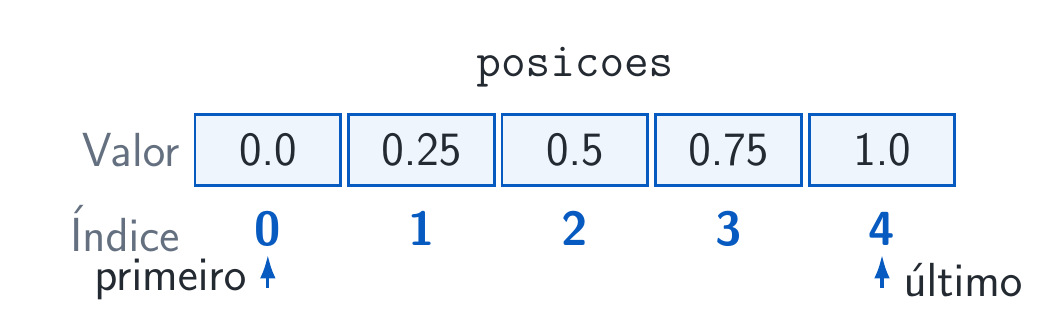
\begin{tikzpicture}[
  x=1cm,y=1cm,every node/.append style={font=\sffamily\fontsize{18}{22}\selectfont},
  seta/.style={-{Latex[length=3mm,width=2mm]},draw=lnccblue,line width=1.2pt}
]
\path[use as bounding box] (-.15,-1.65) rectangle (12.65,1.8);
\node[text=ink] at (6.8,1.3) {\texttt{posicoes}};
\node[anchor=east,text=muted,font=\sffamily\fontsize{16}{20}\selectfont] at (1.9,.25) {Valor};
\node[anchor=east,text=muted,font=\sffamily\fontsize{16}{20}\selectfont] at (1.9,-.75) {Índice};
\foreach \valor/\indice/\x in {0.0/0/2.9,0.25/1/4.85,0.5/2/6.8,0.75/3/8.75,1.0/4/10.7} {
  \draw[draw=lnccblue,line width=1pt,fill=lightblue] (\x-.925,-.2) rectangle (\x+.925,.7);
  \node[text=ink] at (\x,.25) {\valor};
  \node[text=lnccblue,font=\sffamily\fontsize{18}{22}\selectfont\bfseries] (indice\indice) at (\x,-.75) {\indice};
}
\draw[seta] (2.9,-1.5) -- (indice0.south);
\node[anchor=east,text=ink,font=\sffamily\fontsize{16}{20}\selectfont] at (2.75,-1.4) {primeiro};
\draw[seta] (10.7,-1.5) -- (indice4.south);
\node[anchor=west,text=ink,font=\sffamily\fontsize{16}{20}\selectfont] at (10.85,-1.4) {último};
\end{tikzpicture}
\end{document}
